\problemname{Pitch Performance}

\noindent
After a recent disaster at the Easter party karaoke, you are working
on improving your singing. To gauge how well you are doing, you would
like to measure how much the pitch and timing of your singing differs
from the target melody you were trying to perform.

We model the melody in a simplified manner as a piecewise-constant
function $f$, where at time $x$ the melody has pitch $f(x)$. In other
words from time $0$ up to some time $x_1$, $f(x)$ is some constant
value $y_1$, and then at time $x_1$ it changes to some other value
$y_2$ and remains at that value until some time $x_2 > x_1$, and so
on.

Your voice, on the other hand, is of a more wavering nature, and you
may generally not be able to hold an exact constant pitch for any
period of time, sometimes breaking off into an unwelcome falsetto and
sometimes croaking on those low tones.  The pitch of your
voice can be modeled in a highly simplistic way as a
piecewise-quadratic function $g$. In other words from time $0$ up to
$x_1$ (not necessarily the same $x_1$ as for the function $f$), your
pitch $g(x)$ agrees with some quadratic polynomial, and then from time
$x_1$ to $x_2$ with some other quadratic polynomial, and so on.

The difference between your performance $g$ and the target melody $f$
is the area between these two functions.  See Figure~\ref{fig:pitch}
for an example.  Given the melody $f$ and your performance $g$,
compute their difference.

\begin{figure}[h]
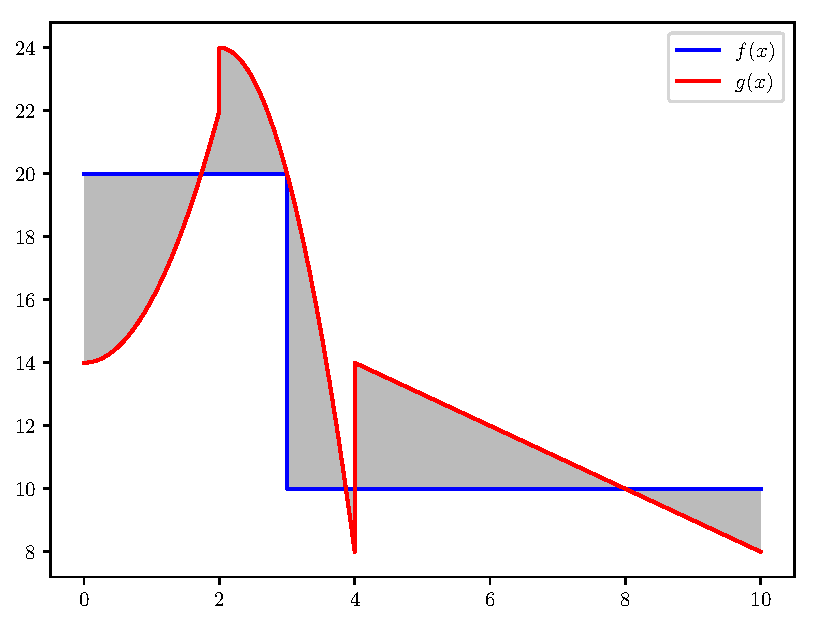
\includegraphics[width=0.73\textwidth]{sample1.pdf}
\centering
\caption{Illustration of Sample Input 1.  The difference between $f$ and $g$ is the area of the shaded region in the figure.}
\label{fig:pitch}
\end{figure}

% Compute the integral $\int_{x=0}^T |f(x)-g(x)| \textrm{d}x$.


\section*{Input}

The first line of input contains an integer $n$ ($1 \le n \le
500$), the number of pieces in the target melody function $f$.  Then follow $n$
lines describing $f$.  The $i$'th such line contains two integers
$x_i$ and $y_i$ ($x_{i-1} < x_i \le 10^4$ and $0 \le y_i \le 10^4$).  For
all $x$ in the half-open interval $[x_{i-1}, x_i)$, the value of
$f(x)$ equals $y_i$.  For the first interval we define $x_0 = 0$.

Then follows a line containing an integer $m$ ($1 \le m \le
500$), the number of pieces in the function $g$ describing your
performance.  The next $m$ lines contain the description of $g$.  The
$i$'th such line contains four integers $x'_i$, $a_i$, $b_i$ and $c_i$
($x'_{i-1} < x'_i \le 10^4$ and $-10^{7} \le a_i, b_i, c_i \le 10^{7}$).
For all $x$ in the half-open interval $[x'_{i-1}, x'_i)$, the value of
$g(x)$ equals $a_ix^2 + b_ix + c_i$.  For the first interval we define
$x'_0 = 0$.

You may assume that $0 \le g(x) \le 10^4$ for all $x'_0 \le x \le
x'_m$ and that the two functions end at the same time (i.e., $x_n =
x'_m$).

\section*{Output}

Output the difference between $f$ and $g$.  Your output should be
correct to within an absolute or relative error of at most $10^{-6}$.
